\documentclass[portuguese]{textolivre}

% metadata
\journalname{Texto Livre}
\thevolume{18}
%\thenumber{1} % old template
\theyear{2025}
\receiveddate{\DTMdisplaydate{2024}{11}{5}{-1}}
\accepteddate{\DTMdisplaydate{2025}{1}{15}{-1}}
\publisheddate{\DTMdisplaydate{2025}{3}{18}{-1}}
\corrauthor{Rafaela Lemos Sales}
\articledoi{10.1590/1983-3652.2025.55719}
%\articleid{NNNN} % if the article ID is not the last 5 numbers of its DOI, provide it using \articleid{} commmand 
% list of available sesscions in the journal: articles, dossier, reports, essays, reviews, interviews, editorial
\articlesessionname{dossier}
\runningauthor{Sales e Ribeiro}
%\editorname{Leonardo Araújo} % old template
\sectioneditorname{Hugo Heredia Ponce}
\layouteditorname{João Mesquita}

\title{O uso de um ambiente imersivo para promover aprendizagem de vocabulário de inglês como língua estrangeira}
\othertitle{The use of an immersive environment to promote English as a foreign language vocabulary learning}

\author[1]{Rafaela Lemos Sales~\orcid{0000-0003-2272-8847}\thanks{Email: \href{rafaelalemos834@yahoo.com.br}{rafaelalemos834@yahoo.com.br}}}
\author[1]{Patrícia Nora de Souza Ribeiro~\orcid{0000-0003-1713-0445}\thanks{Email: \href{mailto:patnora.souza@gmail.com}{patnora.souza@gmail.com}}}

\affil[1]{Universidade Federal de Juiz de Fora (UFJF), Faculdade de Letras, Departamento de Línguas Estrangeiras Modernas, Juiz de Fora, MG, Brasil.}

\addbibresource{article.bib}

%\usepackage{calc,easyReview,enumitem,threeparttable}

\begin{document}
\maketitle
\begin{polyabstract}
\begin{abstract}
Dispositivos tecnológicos estão cada vez mais presentes no ensino,
culminando, mais recentemente, no uso de ambientes imersivos como
ferramentas pedagógicas. Nesse contexto, esta pesquisa objetiva
investigar o uso de um ambiente imersivo em 360º para promover atenção e
motivação nos alunos durante a aprendizagem de vocabulário de inglês
como língua estrangeira (LE). No plano teórico, o estudo é fundamentado
pela \emph{Noticing Hypothesis} \cite{schmidit1990}, pela Teoria
Motivacional de \textcite{gardner1979,gardner2010} e pela Teoria Cognitiva de
Aprendizagem Multimídia \cite{mayer2001,moreno2007}. Metodologicamente, esta
pesquisa é quase experimental, buscando controlar o uso de um ambiente
imersivo em 360º para a promoção da atenção e da motivação durante a
aprendizagem de vocabulário de inglês como LE. Para tanto, foram
realizados três experimentos com 81 alunos do Ensino Médio de uma escola
pública de Juiz de Fora (MG). Esses alunos foram divididos igualmente em
três grupos e cada grupo foi submetido a uma condição de testagem:
ambiente imersivo em 360º, ambiente de leitura com glossário multimodal
e ambiente imersivo em 360º + ambiente de leitura com glossário
multimodal. Os resultados mostram que houve ganho de aprendizagem nas
três condições de testagem, mas a aquisição lexical dos alunos expostos
à terceira condição foi superior. Conclui-se que isso se deve à
multimodalidade presente no ambiente, que contribuiu para a promoção da
atenção e da motivação, resultando no aprendizado.
  
   
\keywords{Aprendizagem de vocabulário \sep Realidade Virtual \sep
Multimodalidade \sep Atenção \sep Motivação}
\end{abstract}

\begin{english}
\begin{abstract}
  Technological devices have become increasingly present in education,
  recently leading to the use of immersive environments as pedagogical
  tools. In this context, this research aims to investigate the use of a
  360º immersive environment to promote attention and motivation during
  English vocabulary learning. Theoretically, the study is grounded in
  Schmidt\textquotesingle s Noticing Hypothesis \citeyear{schmidit1990},
  Gardner\textquotesingle s Motivational Theory \citeyear{gardner1979,gardner2010}, and Mayer's
  Cognitive Theory of Multimedia Learning \cite{mayer2001,moreno2007}. Methodologically,
  this is a quasi-experimental study designed to control the use of a 360º
  immersive environment to promote attention and motivation during English
  vocabulary acquisition. Three experiments were conducted with 81 high
  school students from a public school in Juiz de Fora, MG. These students
  were equally divided into three groups and each group was exposed to a
  different condition: a 360º immersive environment, a reading environment
  with a multimodal glossary, and a 360º immersive environment + reading
  environment with a multimodal glossary. The results indicate learning
  gains across all three conditions, but students exposed to the third
  condition demonstrated superior lexical acquisition. This improvement is
  attributed to the multimodality of the environment, which helped enhance
  attention and motivation, ultimately leading to better learning
  outcomes.
  


\keywords{Vocabulary learning \sep Virtual Reality \sep Multimodality \sep
Attention \sep Motivation}
\end{abstract}
\end{english}
\end{polyabstract}

\section{Introduction}\label{sec-intro}

Technology-assisted interpreting has experienced exponential growth in
recent years, reflected in the dizzying progress in the development of
information and communication technology (ICT) tools and resources
\cite{gutierrezArtacho2016,mezcua2019}. These innovative
technologies have greatly facilitated the interpretation and
comprehension of texts in different linguistic contexts \cite{olallaSoler2015}. In this sense, computer-assisted interpreting (CAI)
has become crucial in an increasingly globalised and connected society,
playing a pivotal role in breaking down language barriers and
facilitating effective communication in an environment characterised by
cultural and linguistic diversity \cite{mellinger2019,li2021}. In
response to the growing demand for instant online communication and the
need to overcome language limitations in a global environment, CAI has
established itself as an infallible tool for a wide range of
applications, from interpreting international business meetings to
translating multimedia content in real time \cite{fantinuoli2017a,alcaidemartinez2021}.

The integration of technology has revolutionised the way individuals
interact with language, opening new possibilities for increasing the
efficiency and accuracy of text interpretation, both in real time and
asynchronously \cite{gaber2023a,ramirezRodriguez2023}. The development
of ICT tools has led to improvements in natural language processing,
machine translation, speech recognition and other related technologies,
resulting in significant advances in text interpretation \cite{valeroGarces2024}. These tools have been particularly useful in overcoming language
barriers in multicultural environments, facilitating communication
between speakers of different languages and promoting intercultural
understanding \cite{perez2020}.

The use of CAI does, however, present certain difficulties. In the
phraseological domain, understanding idiomatic expressions remains a
significant challenge, as these linguistic constructions can be
particularly difficult to interpret accurately due to their cultural
embeddedness \cite{corpaspastorgaber2021,ramirezRodriguez2022}.
Cultural and contextual differences can lead to inaccurate or ambiguous
translations of these expressions, resulting in misunderstandings and
communication problems. In addition, CAI is often based on pre-defined
algorithms and databases, which can limit its ability to adapt to new
idioms and emerging expressions \cite{ortigoza2024}. This problem
identified in the interpretation of idiomatic expressions by CAI adds to
the previously mentioned challenges in technology-assisted phraseology,
where accuracy and fluency in the interpretation of texts in different
linguistic contexts are key to effective communication. The complexity
of idiomatic expressions, such as idioms, and their culturally
contextual nature require new approaches and specialised tools to
improve the interpretation of such expressions, which represents a
relevant area of research in the development of technology-assisted
phraseology.
\section{Aporte Teórico}\label{sec-aporteteo}

\subsection{Atenção}\label{sec-atencao}

Quando se fala de aprendizagem, há construtos que são essenciais e precisam ser
considerados, pois, sem eles, ela não ocorre. Um desses construtos é a atenção.
Os mecanismos atencionais estão presentes em diversas espécies e resolvem um
problema muito comum: o congestionamento de informações. A todo momento, nosso
cérebro é bombardeado por estímulos de natureza diversa, mas é impossível que
todas elas sejam registradas devido aos recursos limitados de nosso cérebro
\cite{dehaene2022,james1890principles,lima2005,posner1990}. Dessa forma, a atenção é um
mecanismo de extrema importância, pois atua como um filtro e executa a triagem
seletiva dessa ampla gama de estímulos. Logo, em cada estágio do processamento
de informação, nosso cérebro decide quanta importância deve dar a cada estímulo
recebido e aloca recursos somente às informações consideradas mais essenciais.

A atenção é amplamente estudada por diversas áreas do conhecimento e pode ser
mensurada em diferentes níveis, como o anatômico e o cognitivo. Na
Neurociência, ela é um campo de estudo abrangente e pode ser definida de
diferentes formas, sobretudo, como um processo cognitivo complexo que envolve
várias redes neurais e funções cerebrais. \textcite{posner1971,posner1990}
define atenção como um sistema integrado de controle do processamento mental
dividido em três grandes subsistemas: alerta, orientação e atenção executiva. O
alerta nos indica o momento em que devemos permanecer vigilantes, ou seja,
quando é necessário direcionar nossa atenção a um estímulo específico. O de
orientação está associado à escolha dos objetos aos quais devemos dedicar nossa
atenção. O da atenção executiva determina como a informação em questão será
processada, estando ligado à limitação da capacidade de processamento no
sistema de controle executivo, o qual guia, direciona e supervisiona nossos
processos mentais.

Na Linguística, a atenção é mais enfatizada em descrições cognitivas de
desenvolvimento da LE, sobretudo, nas abordagens psicolinguísticas,
sendo a atenção ao \emph{input} vista como essencial para o
armazenamento da informação e para a formação e a testagem de hipóteses
sobre a língua. Nos estudos sobre a ASL, ela é considerada um construto
necessário para que o \emph{input} seja convertido em \emph{intake} e se
torne disponível para posteriores processamentos mentais.

\textcite{schmidit1990,schmidt1993awareness,schmidit2001} investiga a relação entre atenção, processos
controlados (como a consciência) e aprendizagem. Fundamentado nos
princípios da psicologia cognitiva e da neurociência, ele argumenta que
a atenção exerce controle sobre o acesso à consciência. Assim, quando
uma pessoa direciona sua atenção para um estímulo, ela se torna
consciente dele. Para o autor, o grau de consciência do aluno se divide
em três níveis cognitivos fundamentais: 1) percepção
(\emph{perception}), relacionada à representação e à organização mental
dos eventos externos; 2) registro cognitivo (\emph{noticing}), isto é,
notar conscientemente os aspectos formais da língua alvo; e 3)
compreensão (\emph{understanding}), relacionada à reflexão acerca dos
aspectos linguísticos notados conscientemente e à tentativa de
compreendê-los.

A partir disso, ele postula a \emph{Noticing Hypothesis}, segundo a
qual, para que o aprendizado ocorra, o aprendiz deve alocar,
conscientemente, sua atenção aos aspectos linguísticos presentes no
\emph{input} da LE para registrá-los cognitivamente (\emph{noticing}) e
compreendê-los. Logo, percebe-se que a atenção é indispensável para a
transformação do \emph{input} em \emph{intake} durante a aprendizagem de
uma LE, visto que sem ela, não há \emph{noticing} e, consequentemente,
não há aprendizado. Assim, o que acontece no espaço atencional determina
significativamente o curso da aprendizagem e do desenvolvimento da
língua. Contudo, um fator determinante para que o aluno se envolva com a
atividade e, desse modo, direcione melhor seu foco atencional para o
objeto de aprendizagem é a motivação, melhor discutida a seguir.

\subsection{Motivação}\label{sec-motivacao}

A motivação é um componente essencial no emprego dos recursos
individuais para alcançar determinado objetivo. Assim, um indivíduo
motivado apresenta um comportamento ativo e empenhado no processo de
aprendizagem, sentindo a necessidade de aprender e atribuir significado
àquilo que foi aprendido, o que reforça o papel central da motivação no
processo de ensino-aprendizagem, despertando o interesse de diversos
pesquisadores e professores pelo tema, sobretudo na área de ASL.
Pesquisas indicam que a motivação tem um impacto direto na frequência
com que os alunos utilizam estratégias de aprendizagem em LE, na
intensidade de interação com falantes nativos, na quantidade de
\emph{input} recebido na língua-alvo, no desempenho em testes, no nível
de proficiência alcançado e na duração das habilidades linguísticas após
a conclusão dos estudos (Christopher, 1986; Gardner, 1992;Robin; Oxford, 1992 \emph{apud} \textcite{oxford1994language}).

A Teoria Motivacional de \textcite{gardner1979} tem sido um alicerce para o
desenvolvimento de estudos sobre a motivação no processo de aprendizagem
de LE. Ele postula que a motivação é responsável, entre outras coisas,
pela atenção ao conteúdo ministrado em sala de aula e pela prática do
conteúdo aprendido em contextos informais (fora da sala de aula).
Segundo essa teoria, o sucesso na aprendizagem de LE se baseia na
cognição individual, que envolve inteligência e aptidão linguística, e
em variáveis motivacionais. \textcite{gardner2010} argumenta que a motivação é
essencial para a aprendizagem da LE, visto que alunos motivados aprendem
mais, pois, estando motivados, prestam mais atenção, o que resulta em
mais \emph{noticing}, e isso faz com que níveis mais altos de
consciência e resultados mais significativos de aprendizagem sejam
alcançados. O autor também destaca que a motivação resulta da combinação
de quatro elementos: objetivo, desejo de alcançar o objetivo, atitudes
positivas diante da aprendizagem da língua e esforço.

Além da atenção e da motivação, fatores essenciais para que a
aprendizagem ocorra, deve-se também considerar recursos tecnológicos
enquanto potenciais ferramentas pedagógicas, visto que podem promover
atenção e motivação nos alunos e auxiliar a aprendizagem. Nesse sentido,
um recurso importante é a multimodalidade, melhor discutida a seguir.

\subsection{Multimodalidade}\label{sec-multimodalidade}

Com a evolução das tecnologias digitais e o advento e a relativa
democratização de dispositivos móveis, o uso de aparatos tecnológicos
com fins pedagógicos se torna cada vez mais viável e diversificado, o
que pode favorecer o ensino e a aprendizagem através da multimodalidade
presente em ambientes digitais. Dessa forma, é pertinente entendermos
melhor como ela pode ser integrada ao ensino de LE, mais especificamente
de vocabulário.

A multimodalidade é um dos componentes da hipermodalidade, que combina
hipertextos com recursos multimodais. Essa combinação permite apresentar
informações de várias formas e organizar o conteúdo de maneira não
linear, integrando diferentes modalidades e promovendo a interação entre
o aprendiz e o material pedagógico \textcite{braga2004}. Nesse sentido, neste
estudo, enfocaremos a multimodalidade para investigar o potencial de
ambientes imersivos como mediadores do processo de ensino e
aprendizagem, entendendo que ela está presente também em ambientes
hipermodais. \textcite{leeuwen2015} define a multimodalidade como um
fenômeno, segundo o qual quase todo discurso é multimodal. Ele
compreende a multimodalidade como a combinação e a integração de
diferentes modos semióticos em determinada instância ou tipo de
discurso.

A multimodalidade, ao permitir que o aluno faça a seleção, a conexão e a
relação entre as informações multimodais apresentadas, partindo de seus
interesses, necessidades e estilos cognitivo e de aprendizagem, pode
potencializar a aprendizagem de LE. Logo, ambientes multimodais de
aprendizagem podem motivar os alunos e fazer com que engajem mais nas
atividades, tornando esse processo mais prazeroso e promovendo uma
aprendizagem mais significativa. Nessa direção, surgem modelos e teorias
de aprendizagem multimodal, sendo os cognitivistas mais comumente
utilizados na investigação desse processo, principalmente aqueles
mediados por computadores e dispositivos móveis.

Entre as teorias e os modelos cognitivistas de processamento da
informação na literatura, destaca-se a Teoria Cognitiva de Aprendizagem
Multimídia\footnote{Em sua teoria, \textcite{mayer2001} utiliza o termo
\emph{multimídia} em vez de \emph{multimodalidade} para se referir ao
uso simultâneo de palavras e imagens. Porém, é comum vermos na
literatura esses termos sendo utilizados como sinônimos. O próprio
Mayer, em trabalho posterior \cite{moreno2007}, ao passar a usar
o termo \emph{multimodalidade} em vez de \emph{multimídia}, sugere que
esses termos podem ser utilizados de forma intercambiável. No entanto,
neste trabalho, priorizaremos o uso do termo \emph{multimodalidade}
por entendermos mídias como ``simplesmente meios, isto é, suportes
materiais, canais físicos, nos quais as linguagens se corporificam e
pelos quais transitam.'' \cite[p.~77]{santaella2007linguagens}, enquanto entendemos
modalidades como subjacentes à multiplicidade dos sistemas sígnicos, a
partir das quais, por processos de combinações e misturas de
diferentes modos (verbais e não verbais), originam-se diferentes
formas de linguagem e processos de comunicação.} \cite{mayer2001}, a qual
sugere que o processamento da informação ocorre em dois sistemas
separados: o visual e o verbal. Porém, essa teoria, apesar de possuir
orientação cognitivista e ter sido inicialmente desenvolvida para
facilitar a compreensão de informações científicas, tem sido amplamente
aplicada, por conta de sua natureza abrangente, na compreensão e na
elaboração de materiais instrucionais em outras disciplinas e áreas do
conhecimento, como a ASL, mais especificamente, na aprendizagem de
vocabulário de LE mediada por tecnologias digitais \cite{souza2004,procopio2016,monteiro2021}.

Segundo o modelo de aprendizagem proposto por \textcite{mayer2001}, palavras
entram no sistema cognitivo por meio dos ouvidos (em caso de palavras
faladas) e imagens entram por meio dos olhos. Na seleção de palavras e
imagens, o aprendiz presta atenção a determinadas palavras e aspectos da
imagem, o que desencadeia a construção do som da palavra e da imagem na
memória de trabalho. Na organização, o aprendiz mentalmente organiza as
palavras e as imagens selecionadas em representações coerentes na
memória de trabalho, o que o autor chama, respectivamente, de modo
verbal e modo imagético. Por fim, na integração, o aprendiz mentalmente
integra esses dois modos ao conhecimento prévio na memória de longo
prazo. Assim, ocorre o aprendizado da informação multimodal à qual o
aprendiz foi exposto. Logo, a teoria propõe que se aprende melhor com
palavras e imagens que apenas com palavras, pois utilizar dois canais
para apresentar a informação (verbal e visual) é como apresentar o
material duas vezes, expondo o aluno duas vezes mais ao conteúdo alvo.

Considerando o papel central da atenção e da motivação no ensino e
aprendizagem de LE, além do uso de tecnologias digitais como mediadoras
desse processo, nossa hipótese é que a multimodalidade presente em
ambientes digitais é um recurso com grande potencial para promover e
facilitar a aprendizagem. Ela pode tornar o processo de aprendizagem
mais agradável e eficiente ao motivar os alunos durante as atividades e
ajudá-los a direcionar melhor sua atenção ao objeto de aprendizagem para
registrá-lo cognitivamente (\emph{noticing}) e, consequentemente,
aprendê-lo. Porém, não são encontrados na literatura modelos e teorias
de ASL que considerem em suas abordagens a atenção e a motivação de
forma integrada e como elementos centrais do processo de aprendizagem de
LE, pois esses construtos, quando abordados, o são de forma periférica e
não integrada \cite{krashen1985,ellis1997,gass1997,hede2002,mayer2002,moreno2007,saito2015,monteiro2021}. Logo,
surge a necessidade de modelos e teorias que integrem esses construtos
caros à aprendizagem de línguas e os considere como centrais nesse
processo.

\section{Metodologia}\label{sec-metodologia}

Não foi necessária uma análise ética prévia por parte dos conselhos de
projetos adequados para a investigação, uma vez que os participantes não
foram identificados. Por não haver conflito de interesses, a Texto Livre
não terá quaisquer consequências, inclusive assistência integral e
eventual, ressarcimento de qualquer dano resultante a qualquer dos
participantes da pesquisa, conforme a Resolução nº 510, de 7 de abril de
2016, do Conselho Nacional de Saúde do Brasil.

A metodologia é a explicação minuciosa, detalhada, rigorosa e exata de
toda a ação desenvolvida no método de trabalho da pesquisa \cite{lakatos2003}. A pesquisa é um estudo de caso, que teve o aluno como
objeto de estudo. \textcite[p. 32]{yin2005} argumenta que o estudo de caso visa a \enquote{conhecer em profundidade o como e o porquê de uma determinada
	situação que se supõe ser única em muitos aspectos, procurando descobrir
	o que há nela de mais essencial e característico}. O estudo de caso é
caracterizado pelo estudo profundo e exaustivo de um ou poucos objetos,
de maneira a permitir o seu conhecimento amplo e detalhado. O caso
experimental caracteriza-se por determinar um objeto de estudo,
selecionar as variáveis que seriam capazes de influenciá-lo, definir as
formas de controle e de observação dos efeitos que a variável produz no
objeto \cite{gil2002}. A coleta dos dados foi realizada em uma escola
secundária do sul de Moçambique. Fizeram parte da amostra 50 alunos do
ensino secundário, selecionados de forma aleatória, dos quais 25
participaram do estudo das PO e aplicação do Q3DM. Os restantes 25
estiveram envolvidos no estudo das SCs e aplicação do GeoGebra. Em ambos
os estudos, todos os alunos experimentaram as aplicações (Q3DM ou
GeoGebra). A pesquisa apresenta um estudo de caso interpretativo, o qual
desenvolve categorias conceituais indutivamente para examinar os
pressupostos iniciais, as intenções e significados das ações e
expressões dos alunos \cite{amado2017}. A compreensão interpretativa é
sustentada a partir do relato pormenorizado da interação dos sujeitos em
seu meio natural \cite{coulon1995}. A visão interpretativa descreveu as
ações dos alunos em ambiente de sala de aula e os significados das ações
no processo de toda a pesquisa \cite{coutinho2011}.

Foi possível, pois, observar e interpretar tudo o que ocorreu, tornando
viável a análise das relações causa-efeito. Foi possível , também,
qualificar as ações dos alunos em todo o processo de aprendizagem, por
meio das interpretações dos significados de seus comportamentos durante
a mediação da aula e as respostas do questionário de satisfação. Além
disso, os dados foram coletados por meio das técnicas de observação do
participante, com tomada de notas e de registro fotográfico, assim como
dos instrumentos de coleta de dados aplicados, como os questionários de
satisfação.

\subsection{Realização das aulas}\label{sub-sec-Realização das aulas}

As aulas consistiram na apresentação de dois temas, PO e SCs, de forma
separada. Para os alunos da 9ª classe, o tema de pesquisa foi PO, e foi
utilizado o Q3DM. A professora primeiramente apresentou o tema,
explicando o que eram POs, dizendo que eram figuras geométricas sobre um
plano que poderiam ser comparadas à sombra do mesmo objeto no horário em
que o sol estaria no ponto mais alto no dia. Depois, demonstrou as
vistas ortogonais do sólido. (Ver \Cref{fig-03}).

\begin{figure}[htpb]
\centering
\begin{minipage}{.5\textwidth}
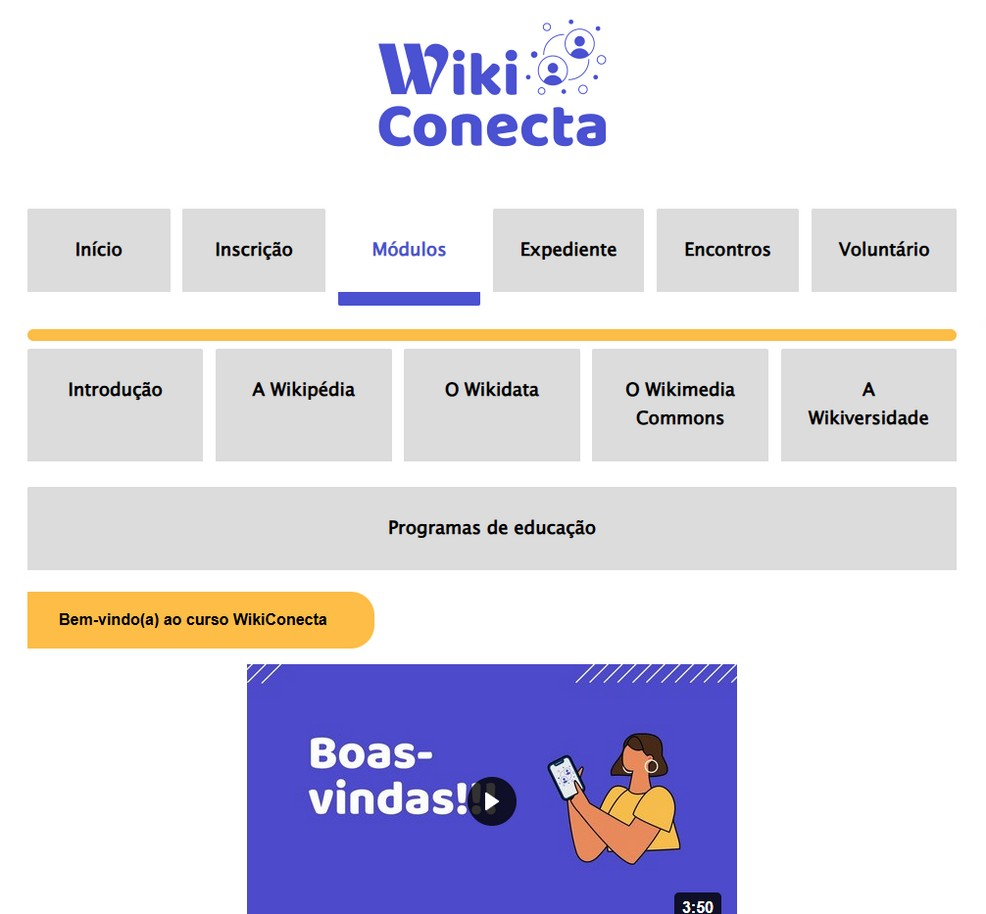
\includegraphics[width=\textwidth]{figures/figure03.jpg}
\caption{Vistas ortogonais e ortográficas: vista frontal; vista superior; e vista lateral esquerda.}
\label{fig-03}
\source{\url{http://turmag1215vialonga.blogspot.com/2014/10/projecoes-ortogonais.html}.}
\end{minipage}
\end{figure}

Posteriormente a professora apresentou a aplicabilidade das POs, dizendo
que eram destinadas à planificação de vários objetos. Com o auxílio das
simulações computacionais, construiu os sólidos geométricos e demonstrou
suas vistas ortogonais, apresentando os procedimentos para a manipulação
do Q3DM. (Ver \Cref{fig-04})

\begin{figure}[htpb]
\centering
\begin{minipage}{.5\textwidth}
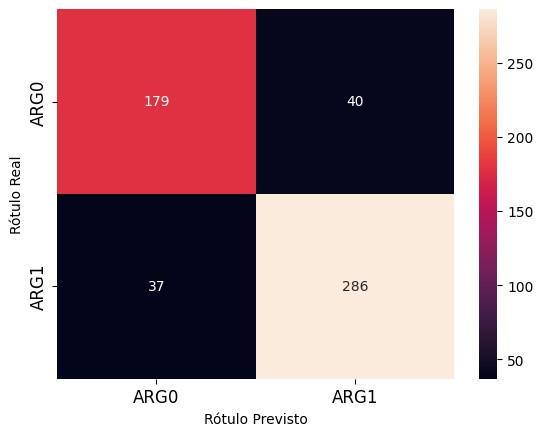
\includegraphics[width=\textwidth]{figures/figure04.jpg}
\caption{Manipulação no Q3DM.}
\label{fig-04}
\source{Elaboração própria.}	
\end{minipage}
\end{figure}


A manipulação no Q3DM é feita por meio de cubos chamados Qubes, que
facilitam a criação e a montagem de objetos em três dimensões,
utilizando elementos digitais que podem ser inseridos, removidos,
deslocados, ampliados, inclinados, moldados geometricamente, girados e
coloridos.

Para os alunos da 12ª classe, o tema de pesquisa foi SCs e foi utilizado
o GeoGebra. A professora iniciou com a apresentação do tema SCs de
cilindro, explicando que a seção cilíndrica é uma figura resultante de
um plano secante no cilindro. A professora acrescentou que existem duas
situações distintas: quando o plano secante é paralelo ao eixo central
do cilindro; e quando o plano secante não é paralelo ao eixo central do
cilindro (ver as figuras \Cref{fig-05} e \Cref{fig-06}).

\begin{figure}[htpb]
\centering
\begin{minipage}{.25\textwidth}
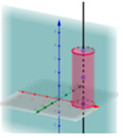
\includegraphics[width=\textwidth]{figures/figure05.jpg}
\caption{Secção paralela ao eixo central do cilindro.}
\label{fig-05}
\source{Elaboração própria.}
\end{minipage}
\end{figure}

\begin{figure}[htpb]
\centering
\begin{minipage}{.5\textwidth}
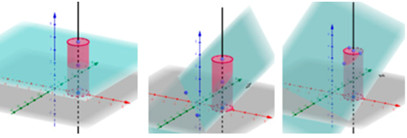
\includegraphics[width=\textwidth]{figures/figure06.jpg}
\caption{Secção não paralela ao eixo central do cilindro.}
\label{fig-06}
\source{Elaboração própria.}
\end{minipage}
\end{figure}

A professora, primeiramente, apresentou os diferentes posicionamentos
dos planos em relação ao eixo central do cilindro. Em seguida, com o
auxílio da tecnologia, apresentou à turma o software de geometria
dinâmica GeoGebra, indicando as funcionalidades de suas ferramentas e
como construir do ponto até o plano secante, com a ajuda dos
procedimentos para a sua manipulação no GeoGebra. Os alunos simularam as
SCs com o plano de nível; eles apresentaram-se atentos e motivados em
aprender a resolver o exercício no GeoGebra, particularmente para os
rapazes, os quais procuravam descobrir como construir diferentes sólidos
geométricos e como simular as VOs (vistas ortogonais).

\subsection{Realização do questionário}\label{sub-sec-Realização do questionário}

O questionário de satisfação aplicado teve como objetivo compreender se
o Q3DM e o GeoGebra facilitaram a aprendizagem das POs e SCs, e se o
\textit{smartphone} foi fácil de manipular. Ambos os questionários foram
preenchidos em 10 minutos. As questões visavam a coletar, nos dois
estudos, várias opiniões, incluindo: (1) se os aplicativos tecnológicos
facilitaram as representações 3D; (2) qual é a opinião deles sobre os
benefícios de usar os aplicativos ou se seria melhor resolver de forma
tradicional; (3) se os aplicativos são fáceis e intuitivos de usar; (4)
quais foram os aspectos positivos e negativos da aula; e, (5) como eles
classificariam a aprendizagem com o auxílio dos aplicativos.

\section{Análise e discussão de dados}\label{sec-analiseediss}

Nos experimentos 1, 2 e 3 os grupos de alunos foram expostos,
respectivamente, ao ambiente imersivo em 360º ao ambiente de leitura com
glossário multimodal e ao ambiente imersivo em 360º + ambiente de
leitura com glossário multimodal. A seguir, esses experimentos serão
melhor discutidos.

\subsection{Experimento 1}\label{sub-sec-experimento1}

Neste experimento, 27 alunos foram expostos ao ambiente imersivo em
360º. Primeiramente, eles utilizaram os \emph{desktops} da escola para
explorar livremente o ambiente. Posteriormente, eles fizeram um
\emph{tour} guiado pela pesquisadora pelas cenas do ambiente, durante o
qual a pesquisadora narrou, interativamente, a peça shakespeariana,
fazendo perguntas aos alunos e direcionando sua atenção para objetos nas
cenas. Tais objetos são relevantes tanto para a história, por se
relacionarem a aspectos centrais da trama, quanto para o experimento,
por serem palavras alvo da atividade de aquisição lexical. Essa narração
interativa foi usada tanto para guiar a exploração dos alunos quanto
para ajudá-los a focar sua atenção nos objetos presentes no
ambiente/palavras alvo do experimento. Destaca-se que as palavras alvo
apareceram no ambiente na modalidade visual, sem apoio do verbal.

Simultaneamente à exploração guiada, os alunos responderam às perguntas
de compreensão, outra forma de salientar as palavras alvo e
apresentá-las aos alunos na modalidade escrita. Assim, cada item lexical
foi apresentado repetidas vezes e através de três modalidades
diferentes: visual, sonora e verbal. Esse reforço dos estímulos é
relevante, pois, como apontam pesquisas na área, apresentar o estímulo
em diferentes modalidades contribui significativamente para o
aprendizado e retenção do vocabulário da LE \cite{chun1996,saito2015,procopio2016,mayer2001,monteiro2021}.

Os resultados obtidos por meio dos testes de vocabulário aplicados aos
alunos antes e após a exposição ao ambiente são evidenciados no \Cref{graph-01}.

\begin{figure}[htpb]
    \centering
    \begin{minipage}{.75\textwidth}
    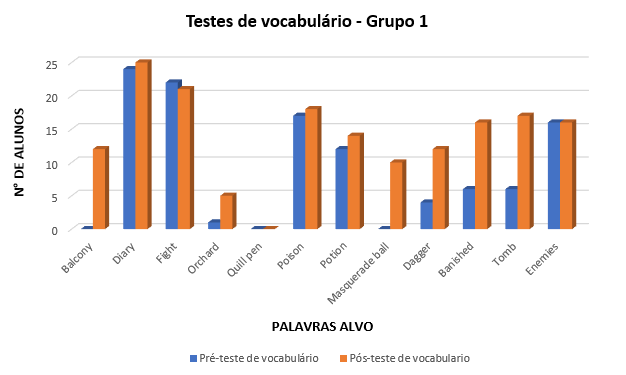
\includegraphics[width=\textwidth]{graph-01.png}
    \caption{Resultado dos Testes de vocabulário do Grupo 1}.
    \label{graph-01}
    \source{Elaborado pelas autoras (2024).}
    \end{minipage}
\end{figure}

Detalhando o gráfico, com base nos dados coletados, percebe-se que o
grupo de alunos exposto ao ambiente de aprendizagem imersivo em 360º
mostrou um ganho de aprendizagem para a maioria das palavras testadas.
Observa-se, entretanto, que algumas palavras tiveram ganho mais
expressivo de aprendizagem após a exposição ao ambiente, como
\emph{balcony, masquerade ball, dagger, banished} e \emph{tomb}
(respectivamente, 44\%, 37\%, 29\%, 37\% e 40\%), enquanto outras
apresentaram um ganho menos expressivo, como \emph{diary, poison} e
\emph{potion} (respectivamente, 4\%, 4\% e 7\%), ou nenhum ganho de
aprendizagem (\emph{fight}, \emph{quill pen} e \emph{enemies}). Essa
diferença pode ser atribuída à importância de cada palavra na narrativa,
pois, apesar de todas serem palavras-chave da tragédia, as que
apresentaram maior ganho de aprendizagem se relacionam diretamente aos
momentos de maior destaque/tensão da narrativa, a exemplo da famosa cena
de Romeo e Julieta na sacada (\emph{balcony}) e do final trágico do
casal na tumba (\emph{tomb}) da família Capuleto.

Conjectura-se que o relativamente baixo ganho de aprendizagem deste
grupo se deve à ausência do verbal (palavra escrita) no ambiente, visto
que apenas a narração não é suficiente para que alunos de nível
elementar consigam inferir o significado das palavras a partir do
contexto e relacioná-las aos objetos presentes no ambiente. Ademais, a
atividade de compreensão realizada durante a exploração do ambiente
também não foi eficaz devido à falta de simultaneidade na apresentação
das modalidades verbal e visual, o que contradiz o Princípio da
Contiguidade \cite{mayer2002} para a elaboração de materiais multimodais.
Segundo este princípio há uma aprendizagem mais profunda quando palavras
e imagens são apresentadas simultaneamente.

Quanto à análise qualitativa, o questionário deste grupo contou com 10
assertivas que visavam avaliar a experiência dos alunos com a atividade,
considerando fatores como usabilidade, engajamento, motivação, atenção e
aprendizagem multimodal. As respostas obtidas podem ser observadas no
\Cref{graph-02}.

\begin{figure}[htpb]
    \centering
    \begin{minipage}{.75\textwidth}
    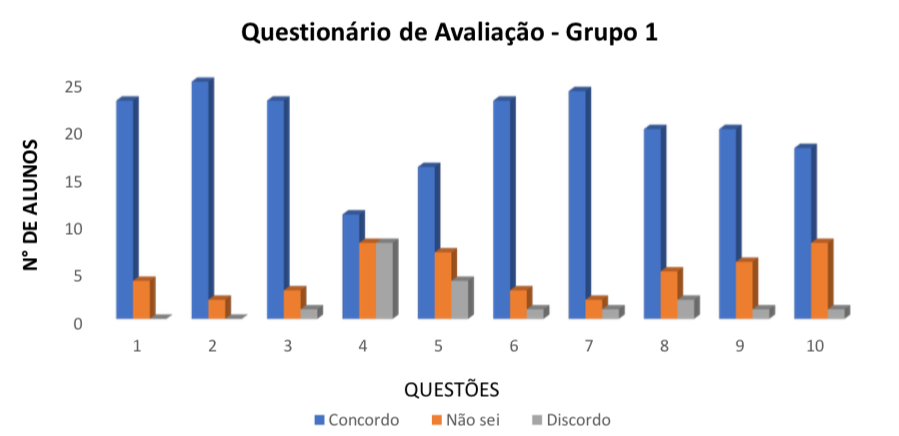
\includegraphics[width=\textwidth]{graph-02.png}
    \caption{Questionário de avaliação da experiência do grupo 1.}
    \label{graph-02}
    \source{Elaborado pelas autoras (2024).}
    \end{minipage}
\end{figure}

A partir das assertivas 1 e 2 (``Usar e interagir com o ambiente foi
fácil para mim'' e ``Aprendi a usar o ambiente de forma rápida e
fácil'') comprova-se a usabilidade do ambiente, visto que 85\% e 92\%
dos alunos, respectivamente, concordaram com elas. Quanto à
aceitabilidade, 85\% concordaram com a assertiva 3 (``A experiência de
aprender vocabulário com ambiente imersivo foi gratificante para mim'').
Quanto ao envolvimento, 41\% afirmaram sentir-se envolvidos durante a
aprendizagem lexical no ambiente, concordando com a assertiva 4 (``Eu me
senti tão envolvido aprendendo vocabulário com o ambiente imersivo que
ignorei tudo ao meu redor''). Esses resultados evidenciam que o ambiente
é fácil e intuitivo de usar, além de favorecer ao engajamento dos alunos
nas atividades. Ele contribui também na criação de um espaço mais
receptivo e motivador para o aprendiz.

As assertivas 5 e 6 averiguaram o direcionamento do foco atencional
proporcionado pelo ambiente. 59\% dos alunos concordaram, 26\% não
souberam responder e 15\% discordaram da assertiva 5 (``O ambiente
ajudou a focar minha atenção nas informações relevantes para a
aprendizagem do vocabulário''). Isso aponta para o potencial do ambiente
enquanto recurso pedagógico, pois ajuda a direcionar a atenção dos
alunos ao objeto de aprendizagem, condição necessária para a ocorrência
do \emph{noticing} (registro cognitivo) e, consequentemente, do
aprendizado \cite{schmidit1990}. Ainda, através da assertiva 6 (``A narração
da professora durante a exploração do ambiente me ajudou a focar a
atenção nos objetos relacionados ao vocabulário''), verificou-se a
pertinência da narração durante o \emph{tour} guiado enquanto estratégia
essencial para ajudar os participantes a focarem sua atenção no objeto
de aprendizagem, como afirmaram 85\% dos alunos.

As assertivas 7 e 8 (``Eu gostei de estudar/aprender vocabulário com
esse ambiente'' e ``Eu me senti mais motivado aprendendo vocabulário com
esse ambiente que com materiais mais tradicionais (ex. livro
didático)''), comprovam a satisfação dos alunos com a aprendizagem
lexical mediada pelo ambiente. Os dados mostram 88\% dos alunos
afirmaram ter gostado de aprender vocabulário através do ambiente e 74\%
concordaram que ele motiva mais que materiais didáticos tradicionais.
Conjectura-se que a multimodalidade presente no ambiente, através da
interatividade e da novidade, é responsável por fazer com que os alunos
se sintam mais motivados em realizar as atividades e, assim, aprender a
LE.

As assertivas 9 e 10 (``Esse ambiente me permitiu compreender melhor o
significado das palavras, podendo ver objetos e relacioná-los à
história'' e ``O ambiente imersivo e os recursos utilizados durante sua
exploração foram suficientes para que eu aprendesse o vocabulário'')
corroboram a efetividade da aprendizagem multimodal, pois 74\% dos
alunos concordaram com a assertiva 9 e 67\%, com a 10, o que ratifica o
papel da multimodalidade como facilitadora do processo de ensino e
aprendizagem, pois a apresentação do material por meio de diferentes
modalidades facilita a compreensão do vocabulário alvo \cite{mayer2001}.

\subsection{Experimento 2}\label{sub-sec-experimento2}

Neste experimento, 27 alunos foram expostos ao ambiente de leitura com
glossário multimodal. Eles ficaram livres para explorá-lo, podendo ler
informações essenciais dos personagens principais e o hipertexto da peça
teatral Romeo e Julieta, cujos \emph{links} (palavras-alvo do
experimento) lhes direcionavam ao glossário multimodal, onde podiam ver
a representação em 2D, a pronúncia e o significado das palavras-alvo.
Não foi feita nenhuma intervenção durante a exploração desse ambiente,
deixando os alunos totalmente livres para navegá-lo e aprender o
vocabulário da forma como preferissem. Os resultados obtidos nos testes
de vocabulário deste experimento podem ser vistos no \Cref{graph-03}.

\begin{figure}[htpb]
    \centering
    \begin{minipage}{.75\textwidth}
    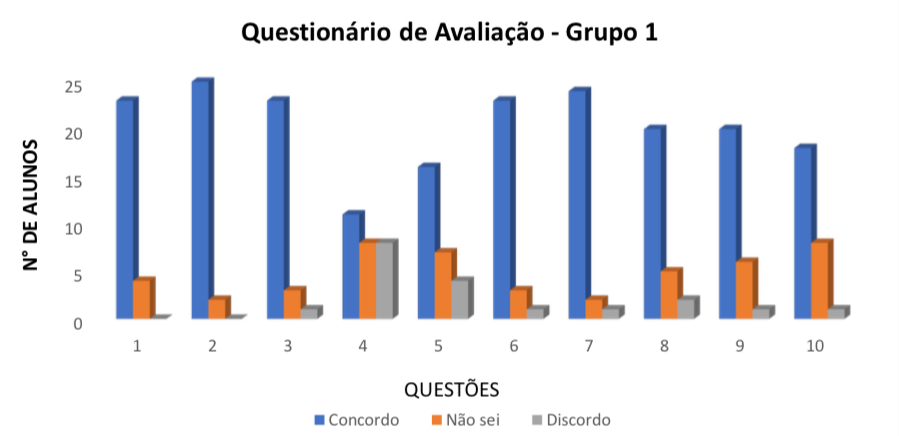
\includegraphics[width=\textwidth]{graph-03.png}
    \caption{Resultado dos Testes de vocabulário do Grupo 2.}
    \label{graph-03}
    \source{Elaborado pelas autoras (2024).}
    \end{minipage}
\end{figure}

Semelhantemente ao experimento 1, o grupo de alunos expostos ao ambiente
de leitura com glossário multimodal também mostrou ganho de aprendizagem
para quase todas as palavras, com exceção de \emph{fight,} e
\emph{enemies}, cujo conhecimento dos alunos antes e após a exposição se
manteve o mesmo. Contudo, percebe-se que, no geral, o ganho de
aprendizagem por palavra foi mais expressivo neste grupo. Por exemplo,
as palavras \emph{quill pen, masquerade ball} e \emph{tomb} apresentaram
um ganho de, respectivamente, 52\%, 52\% e 67\% no experimento 2, mas de
0\%, 38\% e 38\% no grupo 1. Pode-se atribuir essa diferença à presença
da multimodalidade neste ambiente, que se mostra mais eficaz para a
aprendizagem de alunos de proficiência elementar. Isso ocorre porque
este ambiente oferece o apoio do hipertexto e do glossário multimodal,
possibilitando a visualização da forma escrita das palavras-alvo, de seu
significado e imagens correspondentes. Assim, destaca-se a relevância da
apresentação simultânea de palavras escritas e imagem para a
aprendizagem de vocabulário \cite{mayer2001}, visto que as modalidades
verbal e visual são apresentadas aos alunos de forma simultânea.

Já questionário de avaliação da experiência deste grupo possuía 11
assertivas e foi adaptado para contemplar as características do ambiente
de leitura, mas o objetivo foi o mesmo: avaliar a experiência dos
alunos, considerando fatores como usabilidade, engajamento, motivação e
atenção para responder à segunda pergunta desta pesquisa. Os resultados
obtidos podem ser verificados no \Cref{graph-04}.

\begin{figure}[htpb]
    \centering
    \begin{minipage}{.75\textwidth}
    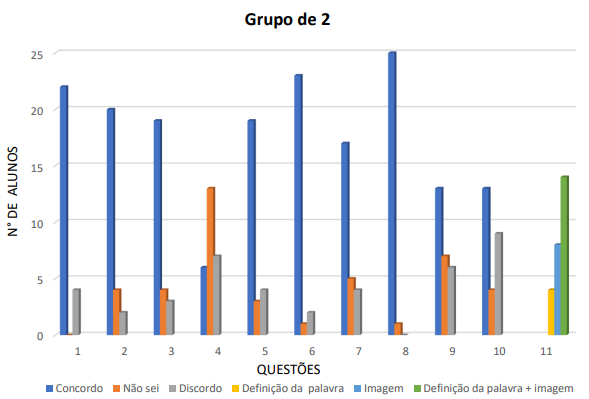
\includegraphics[width=\textwidth]{graph-04.png}
    \caption{Questionário de avaliação da experiência Grupo 2.}
    \label{graph-04}
    \source{Elaborado pelas autoras (2024).}
    \end{minipage}
\end{figure}

Percebe-se que fator usabilidade deste ambiente foi corroborado pelos
alunos, pois 81\% concordaram com a assertiva 1 (``Usar e interagir com
o ambiente foi fácil para mim.'') e 74\%, com a assertiva 2 (``Aprendi a
usar o ambiente de forma rápida e fácil.''). Em relação à
aceitabilidade, 70\% concordaram que a experiência de aprender
vocabulário com o ambiente foi gratificante, fator averiguado através da
assertiva 3 (``A experiência de aprender vocabulário com o glossário
multimodal foi muito gratificante para mim.''). Quanto ao envolvimento
com o ambiente, 22\% concordaram, 52\% não souberam responder e 26\%
discordaram da assertiva 4 (``Eu me senti tão envolvido aprendendo
vocabulário com o glossário multimodal que ignorei tudo ao meu redor).

Quanto à atenção focada, 70\% concordaram com a assertiva 5 (``O
ambiente de leitura com glossário multimodal ajudou a focar minha
atenção nas informações relevantes para a aprendizagem do
vocabulário.''). Assim, evidencia-se que o ambiente ajuda o aluno a
direcionar sua atenção ao objeto de aprendizagem, o que, segundo a
\emph{Noticing Hypothesis} \cite{schmidit1990}, é necessário para ocorrer o
\emph{noticing}. Logo, o ambiente se mostra um recurso pedagógico de
relevância, pois ajuda a promover o registro cognitivo das informações,
promovendo a aprendizagem.

Ademais, 85\% concordaram com a assertiva 6 (``Eu gostei de
estudar/aprender vocabulário com o glossário multimodal.''). Isso aponta
para a agradabilidade proporcionada pelo ambiente \cite{schumann1999neurobiology}, a
qual está relacionada a fatores emocionais ligados à aprendizagem da LE,
como a motivação. Essa foi melhor averiguada através da assertiva 7
(``Eu me senti mais motivado estudando vocabulário com o glossário
multimodal que com materiais tradicionais (ex.: livro didático)''), com
a qual 63\% dos alunos concordaram, 22\% não souberam responder e 15\%
discordaram. Isso mostra que o ambiente possui mais potencial para
motivar os alunos durante a aprendizagem de vocabulário que materiais
didáticos tradicionais/lineares. Atribuímos isso à multimodalidade
presente no ambiente, um recurso que, por meio da interatividade e da
novidade, é capaz de fazer com que os alunos se sintam mais motivados
durante a atividade.

Quanto à aprendizagem multimodal, 92,5\% dos participantes concordaram
com a assertiva 8 (``O glossário me permitiu compreender melhor o
significado das palavras do texto por meio de imagens, pronúncias e
definições.''), evidenciando a eficácia da multimodalidade na
aprendizagem de vocabulário. Isso ocorre, pois a combinação de
diferentes modalidades no glossário permite melhor compreensão das
palavras-alvo, como defende a Teoria Cognitiva de Aprendizagem
Multimídia \cite{mayer2001}. Ademais, 48\% dos alunos concordaram com a
assertiva 9 (``O glossário multimodal foi suficiente para que eu
aprendesse o vocabulário.''), enquanto 30\% não souberam responder e
22\% discordaram. Isso mostra que, embora o glossário multimodal seja
eficaz, a utilização de recursos adicionais pode tornar a aprendizagem
lexical em ambientes multimodais ainda mais eficaz. Logo, surge a
necessidade de testar a eficácia da combinação de outras modalidades
além das utilizadas neste ambiente, o que será averiguado no terceiro
experimento.

Por questões técnicas, não foi possível reproduzir a pronúncia das
palavras presentes no glossário. Por meio da assertiva 10 (``\emph{A
impossibilidade de ouvir a pronúncia das palavras no glossário não
prejudicou minha aprendizagem do vocabulário''}), verificou-se se isso
gerou prejuízos à aprendizagem das palavras. 48\% dos alunos afirmaram
que isso não prejudicou a aprendizagem do vocabulário, enquanto 33\%
discordaram dessa assertiva e 19\% não souberam responder. Porém, o som
é um recurso relevante para os aprendizes de nível elementar e, por
isso, em futuras utilizações deste ambiente de aprendizagem, deve haver
um empenho para que todas as modalidades estejam disponíveis para o
pleno uso dos alunos.

Por fim, na assertiva 11 (``Qual dos recursos presentes no glossário
mais contribuíram para sua aprendizagem do vocabulário?''), buscou-se
averiguar qual das modalidades presentes no glossário foi mais eficaz
para a aprendizagem do vocabulário. Assim, 55,5\% dos alunos apontaram
``palavras + imagem'' como o recurso que mais contribui para sua
aprendizagem no ambiente, enquanto 29,5\% apontaram a ``imagem'' e 15\%,
a ``definição da palavra''. Esse resultado também corrobora a Teoria
Cognitiva de Aprendizagem Multimídia \cite{mayer2001}, a qual defende que
se aprende melhor através de palavras e imagens que apenas de palavras.

\subsection{Experimento 3}\label{sub-sec-experimento3}

No experimento 3, 27 alunos foram expostos ao ambiente de aprendizagem
imersivo em 360º + ambiente de leitura com glossário multimodal.
Primeiramente, eles exploraram o ambiente de leitura, podendo, a
qualquer momento, clicar nos \emph{links} e consultar o significado, a
pronúncia e a representação em 2D das palavras-alvo no glossário
multimodal. Isso pode facilitar a compreensão do significado dessas
palavras e constitui outra forma de salientá-las para além das
repetições no texto, pois a saliência é um fator importante para a
retenção lexical na memória a longo prazo \cite{procopio2016,saito2015}.

Após essa livre exploração do ambiente de leitura, os participantes
foram direcionados para o ambiente imersivo em 360º, no qual fizeram um
\emph{tour} pelas cenas do ambiente guiados pela pesquisadora, que
retomou oralmente o enredo de Romeu e Julieta, salientando as
palavras-alvo e direcionando a atenção dos participantes para os objetos
em 360º, também palavras-alvo do experimento. Essa estratégia teve o
intuito de salientar os objetos, pois a plataforma não permite a
inserção das palavras-alvo na modalidade escrita e o destaque desses
objetos para ficarem mais salientes para os alunos. Os resultados
obtidos neste experimento podem ser vistos no \Cref{graph-05}.

\begin{figure}[htpb]
    \centering
    \begin{minipage}{.75\textwidth}
    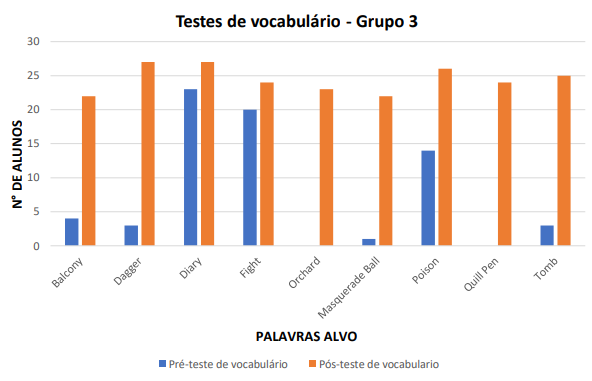
\includegraphics[width=\textwidth]{graph-05.png}
    \caption{Resultado dos Testes de vocabulário do Grupo 3.}
    \label{graph-05}
    \source{Elaborado pelas autoras (2024).}
    \end{minipage}
\end{figure}

Com base nos resultados dos testes de vocabulário dos alunos expostos à
terceira condição de testagem, observa-se um ganho de aprendizagem mais
expressivo para a maioria das palavras em comparação aos dois grupos
anteriores, com destaque para as palavras \emph{dagger, orchard},
\emph{masquerade ball} e \emph{quill pen}, com ganhos de,
respectivamente, 100\%, 73\%, 66\%, 68\% e 63\%.

Esses resultados nos levam a acreditar que, quando os ambientes são integrados,
a aprendizagem lexical é potencializada. Isso se deve aos diferentes recursos
presentes em cada um deles, que, combinados, fazem com que mais modalidades
estejam disponíveis. Isso é corroborado por \textcite{lemke2002}, o qual
postula que o significado das diferentes modalidades é multiplicativo, fazendo
do todo mais que a simples soma das partes e contribuindo, assim, para a
realização de inferências e retenção do significado inferido na memória.
Destaca-se também o fator saliência, essencial para a retenção lexical
\cite{procopio2016,saito2015}, pois o grupo 3 foi exposto a cada uma das
palavras-alvo no mínimo três vezes por meio das modalidades verbal, escrita e
visual.

Quanto à análise qualitativa, devido uma greve docente ocorrida durante
a coleta de dados deste estudo, no início ano de 2024, e à consequente
paralização das atividades do colégio de aplicação em que o experimento
foi aplicado, o questionário de avaliação da experiência deste grupo
precisou ser reduzido e, por isso, diferiu-se dos aplicados aos grupos
anteriores, enfocando mais diretamente a atenção, a motivação e a
aprendizagem multimodal. Através da primeira pergunta discursiva (Você
gostou da atividade? Justifique sua resposta.), averiguou-se que o
ambiente promove a agradabilidade, pois todos os participantes afirmaram
ter gostado da atividade. Segundo \cite{schumann1999neurobiology}, a agradabilidade
promove motivação e engajamento do aluno, facilitando o processo de
aprendizagem. Logo, conclui-se que o ambiente é capaz de promover a
motivação nos alunos durante a aprendizagem de vocabulário.

Na segunda pergunta (Você acha que a atividade te ajudou a aprender
vocabulário?), buscou-se averiguar se a aprendizagem mediada pelo
ambiente é eficaz para a aquisição lexical. Semelhantemente à pergunta
anterior, todos os alunos afirmaram que a atividade ajudou na sua
aprendizagem de vocabulário. Vê-se que o ambiente é capaz de auxiliar os
alunos a direcionarem sua atenção ao objeto de aprendizagem durante a
realização da atividade, promovendo o aprendizado. Isso corrobora a
\emph{Noticing Hypothsis} \cite{schmidit1990}, segundo a qual, para que o
aprendizado ocorra, o aluno deve direcionar sua atenção para o objeto de
aprendizagem para registrá-lo cognitivamente (\emph{noticing}) e
aprendê-lo. Assim, conclui-se que, sem atenção, não há aprendizagem.
Logo, o ambiente, capaz de atrair e direcionar a atenção dos alunos,
mostra-se um recurso pedagógico eficiente para a aprendizagem de LE.

Na terceira pergunta (Qual dos itens abaixo mais contribuiu para o seu
aprendizado de vocabulário durante a atividade?), buscou-se averiguar
qual dos recursos utilizados no ambiente mais contribuiu para a
aprendizagem do vocabulário em LE: a narração do texto; o glossário; a
peça teatral ``Romeu e Julieta''; ou a exploração do ambiente guiada
pela pesquisadora. A opção a mais escolhida foi a exploração guiada do
ambiente (54\%), seguida pelo glossário (27\%), narração (13\%) e peça
teatral (6\%). Logo, conclui-se que o tour guiado pela pesquisadora,
além de suprir limitações do ambiente, mostrou-se um recurso muito
eficaz para a aprendizagem do vocabulário, pois orientou a exploração do
ambiente e direcionou a atenção dos alunos, possibilitando a ocorrência
do \emph{noticing} (registro cognitivo), condição necessária para que o
aprendizado ocorra \cite{schmidit1990}. Além disso, aponta-se a eficácia do
glossário multimodal enquanto recurso que auxilia a aquisição lexical
mediada por ambientes multimodais, pois, além de fornecer um suporte
escrito aos alunos, facilita a aprendizagem ao apresentar o vocabulário
através de diferentes modalidades, o que corrobora a Teoria Cognitiva de
Aprendizagem Multimídia \cite{mayer2001}, pois o uso de duas ou mais
modalidades possibilita que o aluno construa representações mentais mais
ricas e estabeleça relação entre elas, facilitando a aprendizagem.

\section{Conclusão}\label{sec-conclusão}

O presente trabalho apresenta o delineamento da produção de saberes
sobre as TDIC no contexto da Educação Profissional e Tecnológica, mais
especificamente no PROEJA a partir da perspectiva cienciométrica. Como
pode-se observar pelo número de trabalhos retornantes, embora as
tecnologias digitais venham ocupando seu espaço no contexto da sala de
aula, pouco ainda é discutido sobre seu uso por adultos maduros.

Com base nos resultados retornantes, pode-se inferir que as mulheres vêm
se destacando na pesquisa, superando o número de trabalhos desenvolvidos
por homens. Este dado está em consonância com os fomentos para inserção
das mulheres na Ciência e aponta, embora timidamente, para uma conquista
feminina.

A distribuição dos trabalhos quanto a regionalidade, demonstra pequenos
avanços nas políticas de incentivo a descentralização do eixo sudeste,
que em grande parte das áreas de pesquisa se sobressaem em número, pois
é a região com maior número de programas de pós-graduação e de fomento à
pesquisa. Embora não se tenha encontrado nenhum trabalho em programas de
pós-graduação na região norte, uma das dissertações é direcionada ao
público do PROEJA no Instituto Federal de Rondônia (IFRO), o qual fica
situado nesta região.

Quantos aos aspectos metodológicos, pode-se verificar que pelo fato de a
maior parte dos trabalhos ter como origem programas na área de Educação
e Ensino, as pesquisas são, em sua maioria, de caráter qualitativo,
tendo instrumentos de coleta de dados similares e priorizarem a análise
de conteúdo, característica deste campo do saber.

Embora o presente trabalho vise contribuir para sanar a lacuna de
estudos sobre o uso de tecnologias digitais no contexto educacional de
jovens e adultos da educação profissional, o mesmo é apenas uma gota de
água num oceano, visto que a compreensão das necessidades e os desafios
da formação integral que o mundo do trabalho requer não pode ser sanada
sob um único olhar. Neste sentido, aponta-se para a necessidade de
fomentar e incentivar estudos para propiciar o uso das tecnologias
digitais não apenas como elemento de mediação pedagógica, mas também
como possibilidade do desenvolvimento das competências digitais do
cidadão para sua inserção no o mundo do trabalho.

\section{Agradecimentos}\label{sec-agradecimentos}

À CAPES pela bolsa de pesquisa.




\printbibliography\label{sec-bib}
%conceptualization,datacuration,formalanalysis,funding,investigation,methodology,projadm,resources,software,supervision,validation,visualization,writing,review
\begin{contributors}[sec-contributors]
\authorcontribution{Rafaela Lemos Sales}[conceptualization,formalanalysis,methodology,projadm,supervision,writing,review]
\authorcontribution{Patrícia Nora de Souza Ribeiro}[conceptualization,formalanalysis,investigation,methodology,projadm,supervision,review]
\end{contributors}
\end{document}
